%!TEX root = geovis-boilerplate.tex


\begin{abstract}
TODO
\end{abstract}



\section{Introduction}
For decades, computer graphics researchers have strived to achieve the faithful reproduction of reality in synthetic renderings. While photorealism has been achieved in offline rendering contexts, many optical effects occurring in physical environments are still not in use in interactive and real-time applications or implemented with severe limitations. Several lighting effects collectively referred to as ``global illumination'', such as caustics, subsurface scattering and diffuse and specular indirect light, fall into this category.

In this paper, we develop a system that simulates diffuse indirect light in arbitrary and dynamic scenes using many-light techniques. We will trade in quality and instead focus on performance while maintaining scalability with the goal to achieve real-time performance on commodity hardware.




\section{Related Work}

Many-light methods for simulating global illumination effects are a well-researched topic. They are based on Instant Radiosity \cite{Keller:1997:InstantRadiosity}, in which photon mapping is used to create small lights, called Virtual Point Lights (VPLs) at every intersection of photons with the scene geometry.


Most of the work on many-light methods can be categorized into the areas VPL placement, solving occlusion, gathering light into the framebuffer and mitigating singularities, an artifact that occurs near positions of VPLs.


The foundation of many algorithms for VPL placement are Reflective Shadow Maps (RSMs) \cite{Dachsbacher:2005:RSM}, which are shadow maps with additional surface information. Using the additional data, VPLs are created per texel of the RSM. View-adaptive placement of VPLs greatly enhances performance and quality \cite{ritschel2011ismsViewAdaptive}. \cite{prutkin2012reflective} cluster RSM samples to virtual area lights, and \cite{hedman2016sequential} focuses on temporal coherence when placing VPLs to avoid flickering.

A common approach for solving occlusion are Imperfect Sha\-dow Maps (ISMs) \cite{ritschel2008ism}, which use a point-based approximation of the scene to efficiently render a small, approximate shadow map for hundreds of VPLs simultaneously. ISMs have been used in production for rendering many spotlights with shadows \cite{evans2015dreams}, and several enhancements have been proposed \cite{ritschel2011ismsViewAdaptive, hollander2011manylods, barak2013temporally}. Using slim voxels \cite{sugihara2014layered, sun2015manylightsSVO, chen2016quantizing} for occlusion is another approach that needs only a single bit per voxel for visibility testing, thereby avoiding the usually high memory requirements of voxelization techniques.

\cite{dachsbacher2006splatting, Nichols:2009:splatting} are using splatting techniques in favor of the more common gathering approach. \cite{sloan2007image, laine2007incremental} provide details on how to speed up the straight-forward approach of iterating over sets of VPLs per fragment.

In na\"ive implementations of many-light methods, bright spots will appear near the VPL's positions due to the light's attenuation term approaching infinity. A common approach is to clamp the term. This introduces bias, which can be compensated e.g. in screen space \cite{novak2011screen}. Those singularities can also be avoided through more advanced light representations \cite{tokuyoshi2015vsgl}. \cite{olsson2012clustered}



\section{Visibility Computation with Imperfect Shadow Maps}
\label{sec:concept:ism}

The original paper \cite{ritschel2008ism} converts the scene geometry to a point set in a preprocessing step and uses the points to efficiently render hundreds of shadow maps in parallel. They use splatting to render the points and fill the resulting holes in the shadowmaps with a pull-push algorithm inspired by \cite{Marroquim:2007:reconstruction}.

\cite{ritschel2011ismsViewAdaptive} build on this by converting the scene to a triangle texture dynamically, and sampling the points from that texture. Instead of computing a triangle texture, \cite{barak2013temporally} use the tessellation units of recent GPUs to dynamically convert triangles into points.
We follow this approach since it is relatively simple to implement and inherently dynamic, but have not implemented the adaptive sampling from \cite{ritschel2011ismsViewAdaptive} yet.
\cite{ritschel2008ism} also present multi-bounce indirect illumination with their technique, which we have not implemented.

In contrast to \cite{ritschel2008ism}, we have found the pull-push postprocessing to be of little benefit when using regular point splatting. Instead, we propose to render single-pixel points, which opens interesting optimization opportunities but in turn does in fact require the pull-push algorithm to reconstruct the scene surfaces.

We describe the regular point splat rendering process in the following section and subsequently detail the pull-push algorithm that we use when rendering single-pixel points.


\subsection{Point Rendering with Splatting}

To convert the scene to be rendered into points, all its triangles are first tesselated to meet a certain maximum size in order for the point conversion to not introduce extreme inaccuracies. Of the smaller tesselated triangles, the center and area are calulated and a point with matching center and area is created. While it might be more performant to create points just on the vertices of the triangles, it will at the same time be more inaccurate since this approach will enlarge the rendered area considerably over the triangle's extents.

Now a random VPL is chosen per point and backface culling is performed. Likewise, points that lie behind their VPL's hemisphere are culled before splatting the point into the respective imperfect shadow map. For performance reasons, a simple paraboloid projection is used for the ISMs in lieu of conventional cubemaps. Here, another advantage of using points comes into play: Compared to triangles, it is trivial to perform a paraboloid projection on them.

As an optimization, we iterate over several VPLs per point and collect those that pass the culling test and render to all of them. More on this in \cref{chap:implementation}.

To remove holes in the resulting shadowmap, the original paper implements a simplified variant of \cite{Marroquim:2007:reconstruction} that only uses depth information from the point rendering. We found that this approach has little benefit over simply enlarging all the point splats during rendering, therefore we did not use it when using splat rendering.



\subsection{Point Rendering with Pull-Push Postprocessing}

As an alternative to point splat rendering, this subsection proposes a second approach that follows the algorithm of \cite{Marroquim:2007:reconstruction} more closely with the intent to obtain higher-quality shadowmaps. More specifically, the points are rendered as a single pixel, albeit with additional attributes like size and normal. These are then used in a subsequent reconstruction pass to create an (ideally) hole-free shadowmap. This approach also allows a point to be rendered into multiple shadowmaps with a moderate performance impact, more on this in the next chapter.

To provide a rough overview, the pull-push algorithm proposed by \cite{Marroquim:2007:reconstruction} is a ``pyramid-method'' (see \cite{Strengert:2006:Pyramid}) that uses the mipmap levels of a texture to first condense and then spread the data in the texture, in this case the sparse point set representing the scene. During the pull phase, it aggregates the information from four pixels of a finer level to one pixel of a coarser level. The subsequent push phase aggregates four pixels of a coarser level to one pixel of a finer level, but only if the pixel of the finer level contains no data or is determined to belong to an occluded surface. This way, closed surfaces are derived from single-pixel points.

\subsubsection{Pull Phase}
The pull phase reads four pixels of a finer level, computes an aggregate representation of them and writes the result to one pixels of the next coarser level. However, it only considers pixels that pass the following tests: First, they need to contain a valid depth at all (i.\,e.\ a point must have been rendered into this pixel) and second, the point in this pixel must not be occluded. A point is considered to be occluded if it is outside  the depth interval of the frontmost of the four pixel used for interpolation.

Figuratively speaking, the depth interval of a point denotes the range in which other points are considered to belong to the same surface and can be used for interpolation. For the rendered points, the depth interval is simply $[d;d+k]$ where $d$ is the points depth and $k$ an arbitrarily chosen constant. For interpolated points, the new depth interval spans the interpolated depth of the point to the highest depth value of the depth intervals of all ``parent'' points.

To calculate the attributes for a new point, the depth and radius of the parent points are interpolated in between with equal weights. Since the center of the aggregated point might not match with the position of the pixel (this happens if not all four pixels are used for interpolation), a displacement vector is also calculated to accurately describe the point's location.


\subsubsection{Push Phase}

Analogous to the pull phase, the push phase reads four pixels of the coarser level, rejects pixels that don't pass certain tests, and writes one output pixel into the finer level. First, just like in the pull phase, the input pixels must contain a valid depth and not be occluded to be considered. Additionally, a radius check is performed: If the pixel's location is outside the point's extends described by the displacement vector and its radius, then the point is not considered either. This is done to limit a point's influence to its actual size.

The target output location in the finer level might already contain data computed during the pull phase. This data is overwritten if the aggregated data has a smaller depth, i.e. if the original data is considered to be occluded. Otherwise, the original point is left untouched, as it is potentially more accurate than the just computed, interpolated point.

Since the input and output pixel's location do not match the way they do during the pull phase, the weights used for interpolation during the push phase are not uniform, see Figure~\ref{fig:???}.

 \cite{Marroquim:2007:reconstruction} also use the point's normals to correctly limit the point's size, and \cite{Marroquim:2008:reconstruction2} propose gaussian weights based on the pixel's distance to the point's location, instead constant weights solely based on pixel locations. Both of these additions we have not implemented yet.



 \section{ISM Rendering}

 \subsection{Point Rendering with Splatting}




 %\Cref{fig:???} shows the Crytek Sponza scene rendered using ISMs created by the splat renderer (a) and the single-pixel renderer (b). A section of the ISM texture is shown for each renderer in the lower row.


 \subsubsection{Quality}

 \begin{figure}[htb]
 \centering
   \begin{tabular}{@{}cc@{}}
     \includegraphics[width=.22\textwidth]{../screenshots/ism_splat_cropped} &
     \includegraphics[width=.22\textwidth]{../screenshots/ism_single_pixel_cropped}
   \end{tabular}
   \caption{ISMs rendered using the splat renderer (left) and single-pixel renderer (right) with default settings. The single-pixel renderer performs interpolation between points, uses more points and doesn't let points ``bleed'' into neighboring ISMs, but takes more time.}
   \label{fig:results:isms}
 \end{figure}

 \Cref{fig:results:isms} shows a few ISMs rendered with the splat and single-pixel renderer. The imperfections do show, and not only through the low resolutions. The distortion of the surface silhouettes by the splat renderer or postprocessing contribute their part, making it hard to identify which part of the Crytek Sponza is shown.

 \begin{figure}[htb]
 \centering
   \begin{tabular}{@{}cc@{}}
     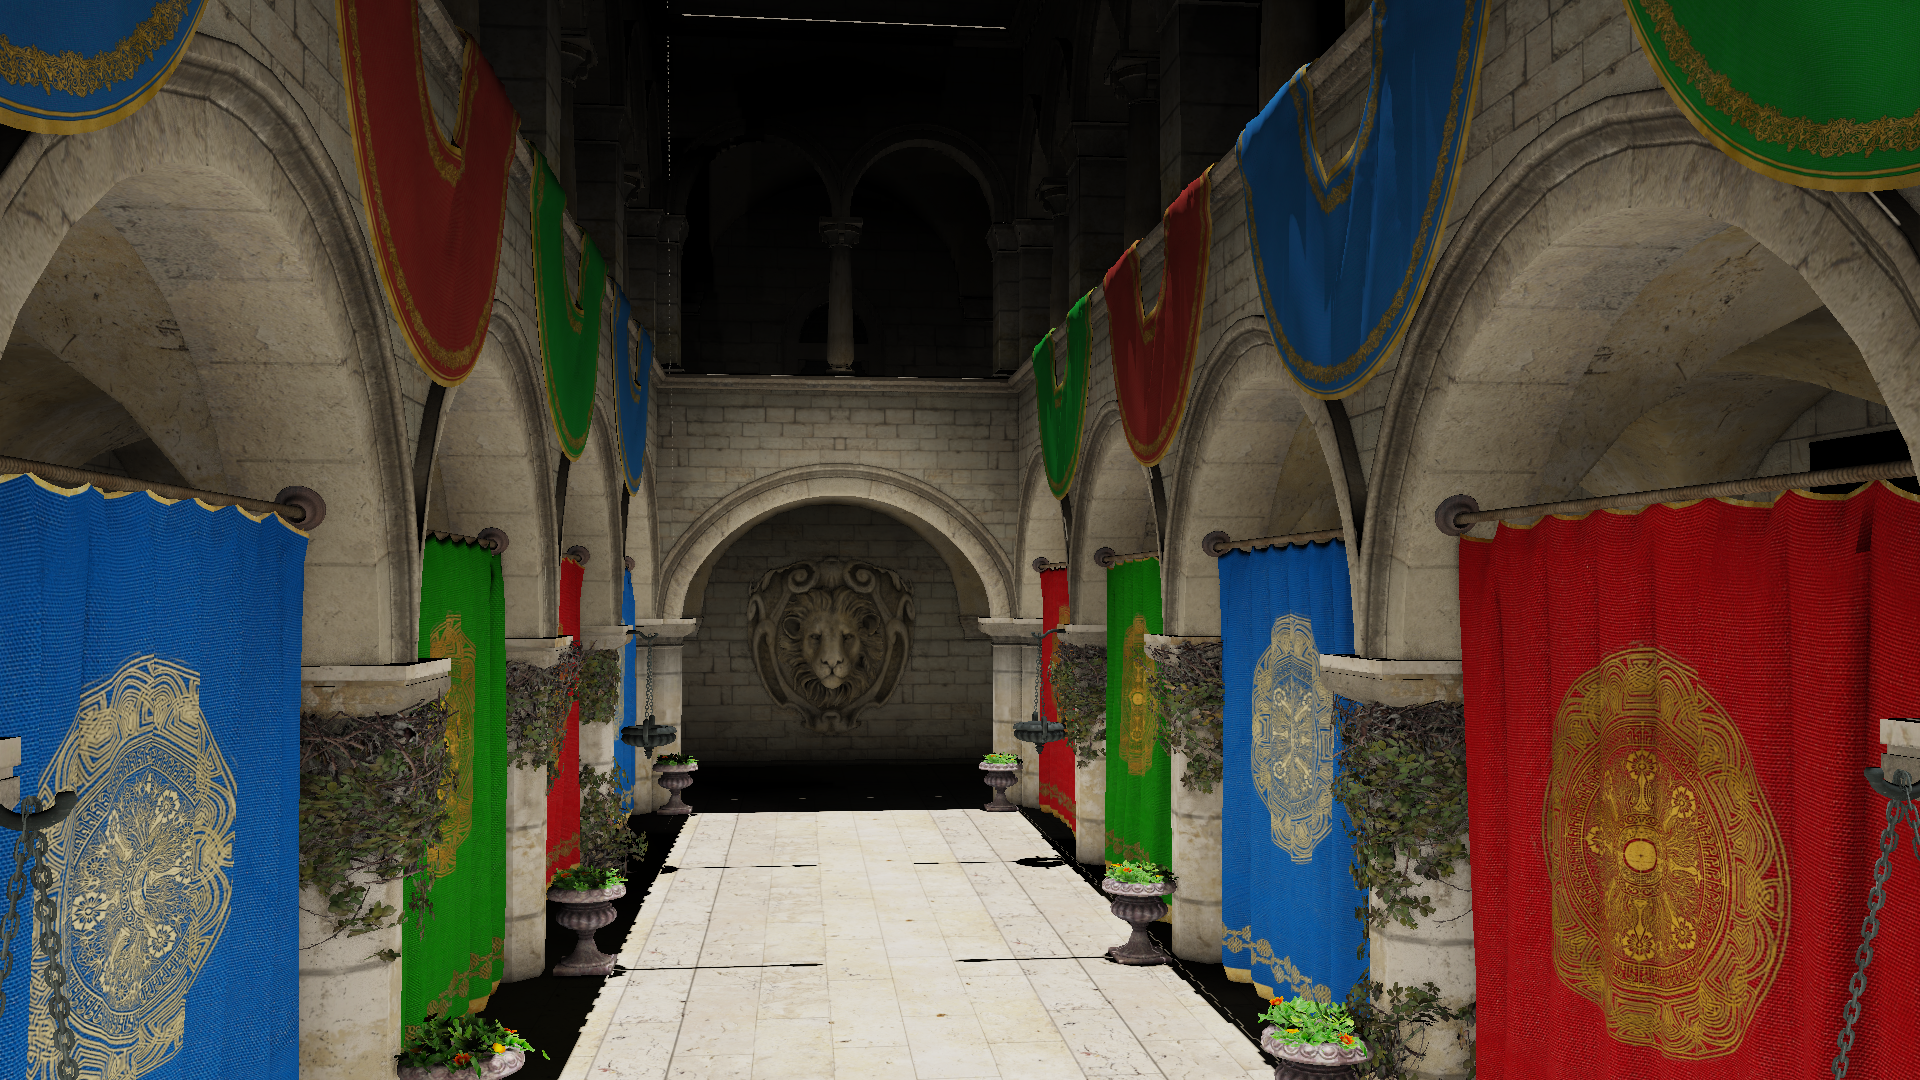
\includegraphics[width=.22\textwidth]{../screenshots/darkening_splat} &
     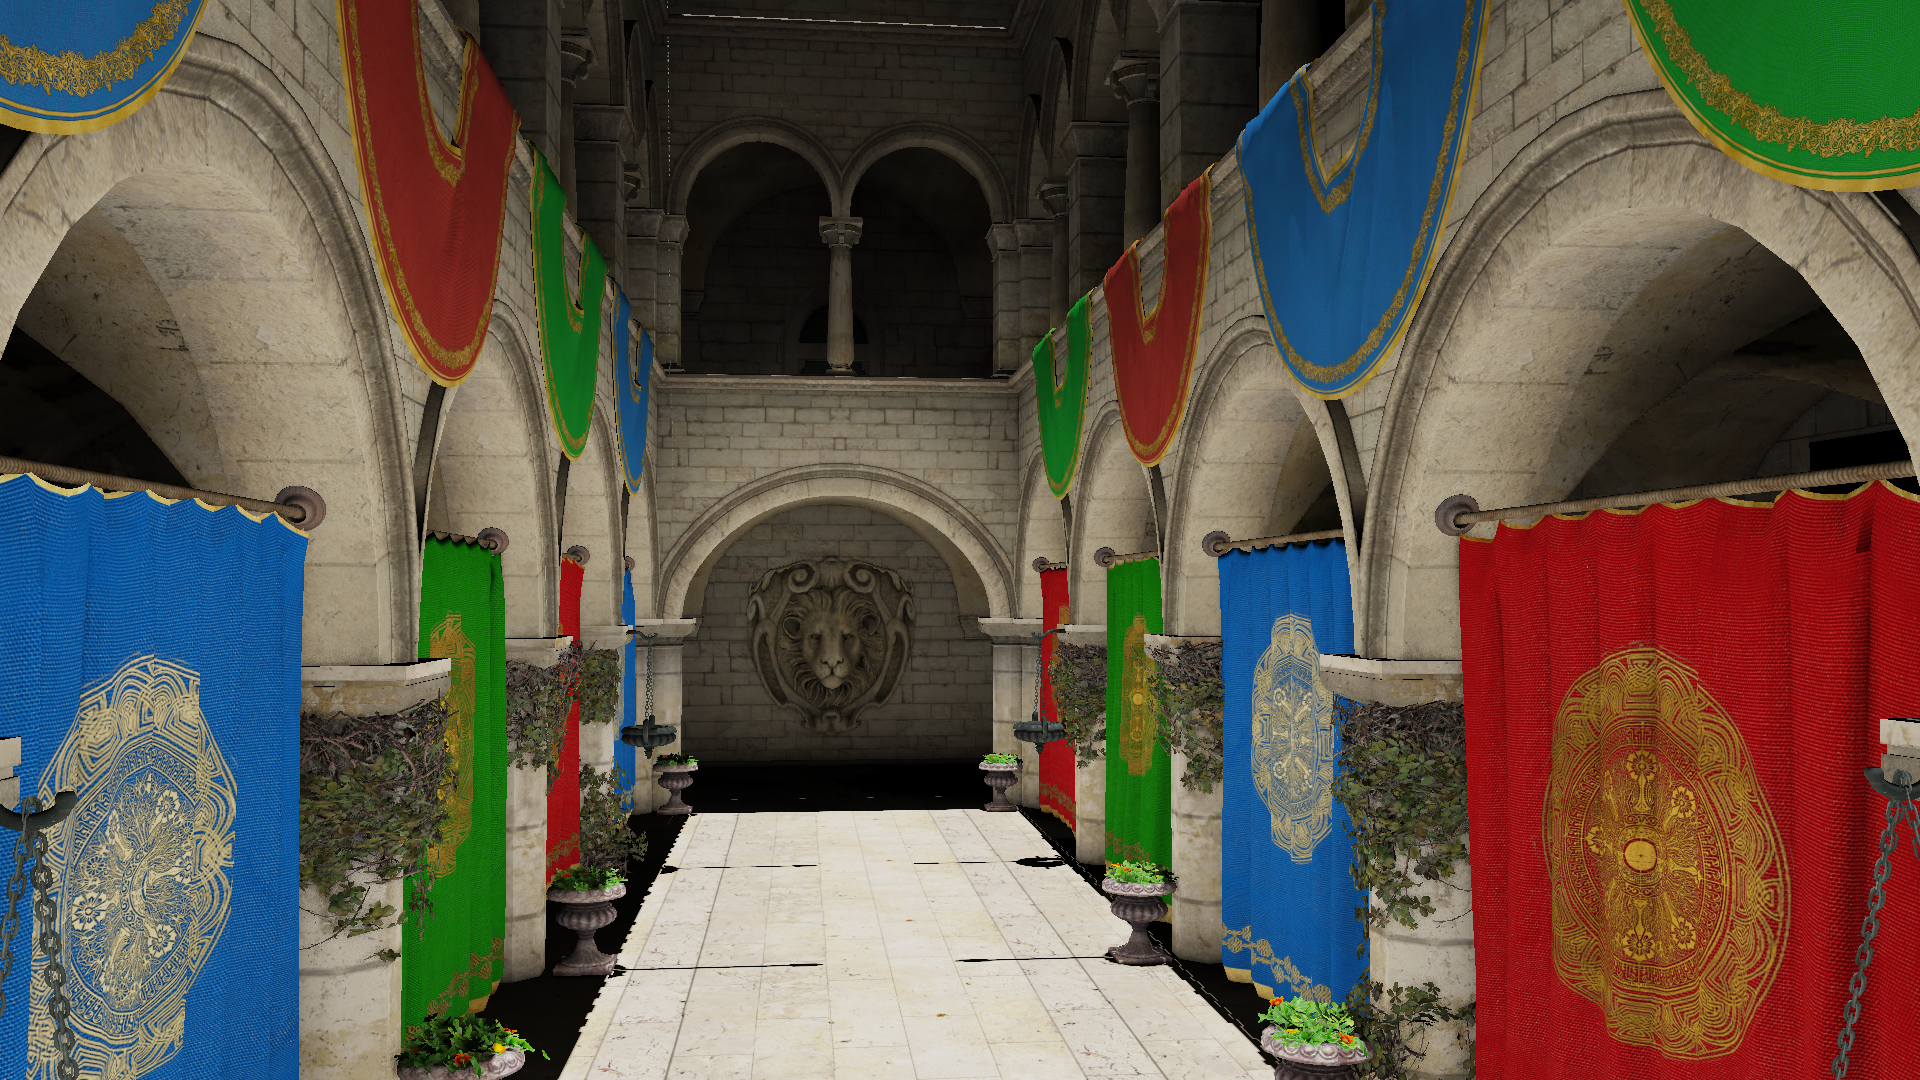
\includegraphics[width=.22\textwidth]{../screenshots/darkening_single_pixel}
   \end{tabular}
   \caption{Darkening caused by the splat renderer (left) compared to the single-pixel renderer (right). Note that there is no skylight rendered, which leads to an unnaturally dark upper part in the image even for the single-pixel renderer.}
   \label{fig:results:ismDarkening}
 \end{figure}

 Comparing the screenshots in \cref{fig:results:ismDarkening}, it becomes apparent that the splat renderer causes visible darkening in the upper part of the image. The reason is likely that the point splats are always oriented towards the camera and do not take the point's normal into account when rendering, amplifying the usual aliasing artifacts of common shadow maps. As a result, any point size larger than one pixel causes surfaces that are not directly facing the camera appear nearer than they actually are when doing shadow lookups in the ISMs. A larger shadow bias could compensate for that but would introduce heavier light leaking. Another possibility would be to use the normal to calculate a point's depth per fragment at a potentially high performance cost.

 As the single-pixel renderer does not use splats, it does not have this problem. One could say it performs the per-fragment depth calculation implicitly during interpolation in the postprocessing phase.


 \begin{figure}[htb]
 \centering
   \begin{tabular}{@{}cc@{}}
     \includegraphics[width=.22\textwidth]{../screenshots/leaks_splat} &
     \includegraphics[width=.22\textwidth]{../screenshots/leaks_single_pixel}\\
     \includegraphics[width=.22\textwidth]{../screenshots/leaks_splat_exposure} &
     \includegraphics[width=.22\textwidth]{../screenshots/leaks_single_pixel_exposure}
   \end{tabular}
   \caption{Light leaks caused by the imperfect shadow maps rendered with the splat renderer (left) and single-pixel renderer (right). VPLs from beneath the curtains leak light onto the wall and ceiling, while VPLs on the pillars and curtains light the floor. The renderings in the bottom row use a higher exposure for illustration. }
   \label{fig:results:leaks}
 \end{figure}


 \Cref{fig:results:leaks} shows a case the ISM technique has difficulties with. The image should be mostly dark or at least uniformly lit through the small gap below the curtains, but  since The root cause for the light problem is that the VPLs are placed right behind the curtains, so the occluding geometry, i.\,e.\ the curtain, is very near to the light source. Due to the randomness involved when selecting the point set for rendering the ISM, it often happens that the points near to the light source are rendered into other ISMs, leaving a large hole behind. The single-pixel renderer copes a bit better than the splat renderer since it uses more points, but does not provide a satisfactory result either.



 \begin{figure}[htb]
 \centering
   \begin{tabular}{@{}cc@{}}
     \includegraphics[width=.22\textwidth]{../screenshots/bias_splat} &
     \includegraphics[width=.22\textwidth]{../screenshots/bias_single_pixel}\\
       \includegraphics[width=.22\textwidth]{../screenshots/bias_splat_exposure} &
       \includegraphics[width=.22\textwidth]{../screenshots/bias_single_pixel_exposure}
   \end{tabular}
   \caption{Light leaks caused by using a relatively large shadow bias with the purpose to hide artifacts of the ISMs. The screenshots to the left use the splat renderer, the right ones the single-pixel renderer. Bottom row uses a higher exposure.}
   \label{fig:results:bias}
 \end{figure}

 Our implementation hides some of the inaccuracies of the ISMs by using a relatively large shadow bias. The resulting light leaks are shown in \Cref{fig:results:bias}. While the splat renderer fares better here, it does so mainly by darkening the whole image since it uses rather large points. The single-pixel renderer on the other hand correctly lets light shine through the columns, but shows a very noisy result on the left wall.















 \subsubsection{Performance}

 \begin{table}[h]
 \begin{center}
     \begin{tabulary}{0.47\textwidth}{| L | L | L | L |}
         \hline
         Splat Default Settings & Single-Pixel Default Settings & Splat with Single-Pixel Settings & Single-Pixel with Splat Settings \\ \hline
         3.4\,ms & 8.5\,ms & 38\,ms & 6.2\,ms \\
         \hline
     \end{tabulary}
     \caption{Timings of the ISM renderers with different settings.}
     \label{tab:results:ism_timings}
 \end{center}
 \end{table}

 \Cref{tab:results:ism_timings} shows the time needed for rendering the ISMs with both renderers and different settings.

 Note that the comparison between the two renderers with default settings is not a fair one, since the single-pixel renderer uses more points and performs clamping per default. If the splat renderer is changed to behave similarly, it takes one additional millisecond for the clamping, and 33 additional milliseconds for using the same technique to collect VPLs as the single-pixel renderer does. The reason for this heavy slowdown is likely that the single-pixel renderer uses shared memory to load the 16 VPLs once, whereas the splatting renderer has to load all 16 VPLs per invocation, since the fragment shader does not provide access to shared memory.

 Conversely, if the single-pixel renderer does not perform clamping, the push phase needs 0.3\,ms less (2.4\,ms to 2.1\,ms), and when it considers only one VPL per point, the compute shader renderer uses 2.0\,ms less (2.9\,ms to 0.9\,ms).

 Since the technique implements no adaptivity, these numbers are independent from the viewport. They are however slightly affected by VPL placement, since it influences culling. In a second scenario, where the sunlight shines directly from above, all VPLs are placed on the floor facing up. As a result, much fewer points are culled during ISM rendering, resulting in slightly higher timings. The splat renderer needed an additional 0.7\,ms, whereas the single-pixel renderer needed only 0.2\,ms more.






 \subsubsection{Detailed Performance Measurements for the \\ Single-Pixel Point Renderer}


 \begin{table}[h]
 \begin{center}
     \begin{tabulary}{0.47\textwidth}{| L | L | L | L || L |}
         \hline
         Point Collection & Point Rendering & Pull Phase & Push Phase & Total\\ \hline
         2.1\,ms & 3.0\,ms & 1.0\,ms & 2.4\,ms & 8.5\,ms\\
         \hline
     \end{tabulary}
     \caption{Timing breakdown of the single-pixel point renderer.}
     \label{tab:results:timing_breakdown_single_pixel}
 \end{center}
 \end{table}

 \begin{table}[h]
 \begin{center}
     \begin{tabulary}{0.47\textwidth}{| L | L | L | L | L | L | L | L || L | L || L |}
         \hline
         PL 1 & PL 2 & PL 3 & PL > 3 & PS > 2 & PS 2 & PS 1 & PS 0 & PL Total & PS Total & Total \\ \hline
         0.57 & 0.34 & 0.10 & 0.04 & 0.09 & 0.19 & 0.71 & 1.47 & 1.05 & 2.46 & 3.5\\
         \hline
     \end{tabulary}
     \caption{Timing breakdown of the pull (PL) and push (PS) phase. The numbers of the individual steps indicate to which mipmap level they write, which is why the pull phase starts with 1 and the push phase has descending numbers. All timings are in milliseconds.}
     \label{tab:results:timing_breakdown_pull_push}
 \end{center}
 \end{table}


 \Cref{tab:results:timing_breakdown_single_pixel} gives more detailed performance measurements of the single-pixel renderer, while \cref{tab:results:timing_breakdown_pull_push} further breaks down the individual steps of the pull and push phase. Note how the timings scale roughly as expected (PL 3 and PS 2 are taking roughly 4 times longer than PL 2 and PS 1, respectively), but not so the first and last step. This is due to the reduced input data size (or output size, respectively), as explained in \cref{sec:impl:pullPushPostprocessing}. Also note how the push phase does take roughly the time of the pull phase if it were not for the last phase, where it writes to the full 2048\,px² of miplevel zero, whereas the first pull phase only writes to the miplevel one with 1024\,px².



 % show this is bandwidth bound. calculation how much memory is read and written, vs bandwidth of GTX 980.
 %     - roughly 110MB read and written, that's 1.2ms.
 %     - 16MB of that unnecessarily because of the 2nd layer of input texture
 %     - By parallel reduction juju reduced by 22MB or 0.2ms.
 %     - with more juju, maybe brought down to actually that time, except for the arithmetic stuff of course...


 \subsubsection{Memory Usage}

 The point splat renderer uses no more memory than the ISM texture itself requires, which is 8\,MB for a 2048\,px² 16-bit depth buffer.

 The single-pixel renderer uses additional memory. First, it uses a buffer for storing the points. This is implemented as four-channel 32-bit float texture, with the first three channels containing the position, and the last channel the radius (8 bit) and normal (24 bit, see \cite{Cigolle:2014:NormalPacking}). With a maximum point count of 2048 per ISM (keep in mind they are rendered into multiple ISMs later), this buffer uses 32\,MB.
 The additional textures used are the render target of the single-pixel renderer (single-channel 2048x2048x2\,px, 32-bit integer, uses 32\,MB), the mipmap levels used by the pull-push algorithm (two channels, 32-bit, use approx. 11\,MB) and the final ISM (same as used by the splat renderer, uses 8MB).

 Added together, the single-pixel renderer uses a total of 83\,MB, likely with room for optimization left.


 \subsubsection{Problems with High Geometric Density}

 As a more demanding test case the San Miguel scene with 7.9M triangles. The most apparent problem of the presented implementation is the lack of adaptivity to the current viewport and VPL positions in addition to the lack of LOD methods. As a result, all 7.9M triangles are used every frame to render the ISMs, with corresponding performance results.

 Screenshots with the San Miguel scene

 Quality also suffers. Not tuned to such small triangles.

 Numbers


 \subsection {Comparison of the Splat and Single-Pixel Renderer}

 The single-pixel renderer provides numerous advantages over the splat renderer.

 Using a compute shader to render the points lifts the restrictions of the fixed-function pipeline and e.\,g.\ enabled rendering each point into multiple ISMs without large performance losses.

 Quality-wise, it can reproduce surfaces more accurately by correctly interpolating between points.

 Obviously, the algorithm needs more rendering time and memory.



 Another drawback is the added complexity. Specifically, we found it hard to fine-tune the pull-push algorithm to give us satisfactory results, especially in the face of the low resolutions of ISMs and the limited data available for reconstruction after selecting a random and sparse set of points.

 flexibility, interpolation, no fillrate problem

 but hard to fine-tune



 \subsection{Comparison and Discussion}


 Imperfect shadow maps have several deficits, some of which are inherent to the technique and difficult to solve, others are specific to the implementation choices and tradeoffs in our implementation and might be easier to overcome.

 First, ISMs reduce the scene's geometry to points. At the resolution that is achievable in a real-time budget, this is already a stark approximation that loses a lot of accuracy.

 Second, because a sparse set of points is used for each ISM, each point must be enlarged to accomodate for the neighboring points that are likely missing in the chosen ISM. For instance, if an area is represented by a thousand points and we now use one tenth of all points for an ISM, each remaining point's area must be enlarged by a factor of ten to result in an equally large area in the rendered output. Of course, this approach leads to deformed geometry since points at the edges of the area get enlarged as well, growing over the borders of the original geometry.

 Third, there are also numerical issues. For instance, both the splatting and postprocessing approaches ignore the distortion caused by the projection, and thus might render even simple surfaces incorrectly. This contributes to the necessity of using a relatively large shadow bias. This can likely be solved however, albeit at the cost of additional complexity.

 Fourth, and this is in our view the most important shortcoming, ISMs handle geometry in the vicinity to VPLs badly as can be seen in \cref{fig:results:leaks}. To sufficiently approximate such surfaces when rendering ISMs, one would need to greatly increase the number of points created near VPLs, possibly in addition to stepping away from using a fully random approach for point selection and select a specific point set for each ISM depending on the VPLs location.

 As for most global illumination algorithms, a massive improvement would be to differentiate between large-scale scene geometry that is important for diffuse light bounces, and smaller geometry of lesser importance. While the latter can possibly be ignored altogether with only minor losses in quality, the shape of large-scale geometry is all the more important to preserve (relatively) precisely.

 The San Miguel scene is a good example for this: While the small detail work like dishes and small plants make up most of the geometry and thus most of the rendering time, they contribute only very little to global illumination. This is where our implementation suffers most from the lack of level-of-detail methods.
